\documentclass[12pt,a4paper]{article}
\usepackage[utf8]{inputenc}
\usepackage[T1]{fontenc}
\usepackage{amsmath}
\usepackage{amsfonts}
\usepackage{amssymb}
\usepackage{multicol}
\usepackage{qrcode}
\usepackage{lmodern}
\usepackage{colortbl}%permet de griser les cases
\usepackage{tabularx, multirow}
%\usepackage{lscape}
\usepackage{xcolor}
%\usepackage{graphicx}
\usepackage{tikz,tkz-base}
% Fichier de style stage.sty [UTF8]
% Copyleft Laurent Bretonnière, laurent.bretonniere@gmail.com
% Version du 14/03/2015 

%*********************************************************************************************
% Packages
%*********************************************************************************************

\usepackage[utf8]{inputenc}%			encodage du fichier source (Linux)
\usepackage[TS1,T1]{fontenc}%			gestion des accents (pour les pdf)
\usepackage[french]{babel}%				rajouter éventuellement greek, etc.
\frenchbsetup{CompactItemize=false,StandardLists=true}
\usepackage{enumitem}%
\setenumerate[1]{label=\arabic*/}%
\setenumerate[2]{label=\alph*/}%
%\setlist{font=\bfseries,leftmargin=*}%
\setlist{font=\bfseries,leftmargin=*,topsep=1pt,partopsep=1pt,itemsep=2pt,parsep=1pt}%

\usepackage{textcomp}%					caractères additionnels
\usepackage{amsmath,amssymb}%			pour les maths (1)
\usepackage{amsfonts}%					pour les maths (2)
\usepackage{lmodern}%					remplacer éventuellement par txfonts, fourier, etc.

\usepackage{graphicx}%

% cf site web http://www.khirevich.com/latex/microtype/
%\usepackage[babel=true,kerning=true]{microtype}%
\usepackage{microtype}%

\usepackage{dsfont}%					pour les ensembles de nombres N,Z,D,Q,R,C ...
\usepackage{mathrsfs}%					pour les écritures calligraphiques (genre Cf et Df)
\usepackage[np]{numprint}% page 58  	pour afficher les nombres 3 par 3
\usepackage[e]{esvect}% page 60		vecteurs
\usepackage{stmaryrd}%					pour les intervalles entiers et sslash
\usepackage{empheq}% 					encadrer en mode math
\usepackage{xcolor}%					pour gérer les couleurs
\usepackage{soul}% 						pour les fluos	
\usepackage{xspace}%					gestion des espaces
\usepackage{pifont}% 					trèfle, pique, carreau, coeur
\usepackage{eurosym}%					symbole euro
\usepackage{mathabx}%					choix personnel

\usepackage{hyperref}%
\hypersetup{%
colorlinks=true,%
breaklinks=true,%
citecolor=red,%
urlcolor=blue,%
linkcolor=black,% ou blue
bookmarksopen=false,%
pdfcreator=PDFLaTeX,%
pdfproducer=PDFLaTeX,%
pdfmenubar=true,%
pdftoolbar=true,%
pdfauthor={Laurent Bretonnière},%
pdfkeywords={Mathématiques},%
pdfstartview=XYZ}%

%*********************************************************************************************
% Mathématiques (cf chapitre 7 page 56, LaTeX pour le prof de maths, IREM de Lyon)
%*********************************************************************************************

% Fonctions usuelles
\DeclareMathOperator{\cotan}{cotan}%
\DeclareMathOperator{\ch}{ch}%
\DeclareMathOperator{\sh}{sh}%
\DeclareMathOperator{\thyp}{th}%
\renewcommand{\th}{\thyp}%
\DeclareMathOperator{\Arcsin}{Arcsin}%
\DeclareMathOperator{\Arccos}{Arccos}%
\DeclareMathOperator{\Arctan}{Arctan}%
\DeclareMathOperator{\Argsh}{Argsh}%
\DeclareMathOperator{\Argch}{Argch}%
\DeclareMathOperator{\Argth}{Argth}%
\DeclareMathOperator{\pgcd}{pgcd}%
\DeclareMathOperator{\ppcm}{ppcm}%
\DeclareMathOperator{\card}{card}%

% Composée de fonctions
\newcommand{\rond}{\circ}%

% Multiplication
\newcommand{\x}{\times}

% Constantes usuelles
\renewcommand{\i}{\mathrm{i}}%
\newcommand{\e}{\mathrm{e}}%

% Éléments différentiels
\newcommand{\dt}{\,\textrm{d}t}%
\newcommand{\du}{\,\textrm{d}u}%
\newcommand{\dv}{\,\textrm{d}v}%
\newcommand{\dw}{\,\textrm{d}w}%
\newcommand{\dx}{\,\textrm{d}x}%
\newcommand{\dy}{\,\textrm{d}y}%
\newcommand{\dz}{\,\textrm{d}z}%

% Ensembles de nombres
\newcommand{\ensnb}[1]{\ensuremath{\mathbb{#1}}}%
\newcommand{\N}{\ensnb{N}}%
\newcommand{\Z}{\ensnb{Z}}%
\newcommand{\D}{\ensnb{D}}%
\newcommand{\Q}{\ensnb{Q}}%
\newcommand{\R}{\ensnb{R}}%
\newcommand{\Rp}{\R_{+}}%
\newcommand{\Rm}{\R_{-}}%
\newcommand{\mtsmall}{\fontsize{5pt}{5pt}\selectfont}%
\newcommand{\Rpe}{\R_{\mbox{\mtsmall$+$}}^{\mskip0.4mu\ast}}%
\newcommand{\Rme}{\R_{\mbox{\mtsmall$-$}}^{\mskip0.4mu\ast}}%
\newcommand{\Ret}{\R^{\ast}}% \Re pris pour la partie réelle d'un complexe
\newcommand{\Ne}{\N^{\ast}}%
\newcommand{\Ze}{\Z^{\ast}}%
\newcommand{\C}{\ensnb{C}}%
\newcommand{\Ce}{\C^{\ast}}%

% Noms de points en majuscules en romain (et non pas en italiques)
\DeclareMathSymbol{A}{\mathalpha}{operators}{`A}
\DeclareMathSymbol{B}{\mathalpha}{operators}{`B}
\DeclareMathSymbol{C}{\mathalpha}{operators}{`C}
\DeclareMathSymbol{D}{\mathalpha}{operators}{`D}
\DeclareMathSymbol{E}{\mathalpha}{operators}{`E}
\DeclareMathSymbol{F}{\mathalpha}{operators}{`F}
\DeclareMathSymbol{G}{\mathalpha}{operators}{`G}
\DeclareMathSymbol{H}{\mathalpha}{operators}{`H}
\DeclareMathSymbol{I}{\mathalpha}{operators}{`I}
\DeclareMathSymbol{J}{\mathalpha}{operators}{`J}
\DeclareMathSymbol{K}{\mathalpha}{operators}{`K}
\DeclareMathSymbol{L}{\mathalpha}{operators}{`L}
\DeclareMathSymbol{M}{\mathalpha}{operators}{`M}
\DeclareMathSymbol{N}{\mathalpha}{operators}{`N}
\DeclareMathSymbol{O}{\mathalpha}{operators}{`O}
\DeclareMathSymbol{P}{\mathalpha}{operators}{`P}
\DeclareMathSymbol{Q}{\mathalpha}{operators}{`Q}
\DeclareMathSymbol{R}{\mathalpha}{operators}{`R}
\DeclareMathSymbol{S}{\mathalpha}{operators}{`S}
\DeclareMathSymbol{T}{\mathalpha}{operators}{`T}
\DeclareMathSymbol{U}{\mathalpha}{operators}{`U}
\DeclareMathSymbol{V}{\mathalpha}{operators}{`V}
\DeclareMathSymbol{W}{\mathalpha}{operators}{`W}
\DeclareMathSymbol{X}{\mathalpha}{operators}{`X}
\DeclareMathSymbol{Y}{\mathalpha}{operators}{`Y}
\DeclareMathSymbol{Z}{\mathalpha}{operators}{`Z}

% Raccourci displaystyle + hack :-)
\newcommand{\dps}{\displaystyle}%
\newcommand{\dsp}{\displaystyle}%
\newcommand{\disp}{\displaystyle}%
\everymath{\displaystyle}%

% Mots usuels en mode math
\newcommand{\mtext}[1]{\quad\text{#1}\quad}%
\newcommand{\et}{\mtext{et}}%
\newcommand{\ou}{\mtext{ou}}%
\newcommand{\si}{\mtext{si}}%

% Flèches
\newcommand{\tv}{\shortrightarrow}% tend vers
\renewcommand{\to}{\shortrightarrow}% tend vers
\newcommand{\suit}{\hookrightarrow}% X suit la loi...
\newcommand{\dans}{\longrightarrow}% f:\R\dans\R
\newcommand{\donne}{\longmapsto}% f:x\donne 2x+3
\newcommand{\ppv}{\leftarrow}% flèche <-- d'affectation "prend pour valeur"
\newcommand{\ech}{\leftrightarrow}% double flèche <--> : échange/swap

% Vecteurs
% \vv{AB} en utilisant l'extension \usepackage[e]{esvect}

% Norme et valeur absolue
\newcommand{\abs}[1]{\left\lvert#1\right\rvert}%
\newcommand{\norme}[1]{\left\lVert#1\right\rVert}%

% Complexes
\renewcommand{\Re}{\operatorname{Re}}
\renewcommand{\Im}{\operatorname{Im}}
\renewcommand{\bar}{\overline}

% Matrices
\newcommand{\trans}[1]{{\vphantom{#1}}^{\mathit{t}}\!{#1}}%

% Coefficient binomial
\newcommand{\cb}[2]{\binom{#2}{#1}}%

% Matrice augmentée
\makeatletter
\renewcommand*\env@matrix[1][*\c@MaxMatrixCols c]{%
  \hskip -\arraycolsep
  \let\@ifnextchar\new@ifnextchar
  \array{#1}}
\makeatother

% Parallèles et perpendiculaires
\newcommand{\para}{\sslash}%
% perp pour perpendiculaire

% Intervalles
\newcommand{\intervalle}[4]{\mathchoice%
{\left#1#2\mathclose{}\mathpunct{},#3\right#4}% mode \displaystyle
{\mathopen{#1}#2\mathclose{}\mathpunct{},#3\mathclose{#4}}% mode \textstyle
{\mathopen{#1}#2\mathclose{}\mathpunct{},#3\mathclose{#4}}% mode \scriptstyle
{\mathopen{#1}#2\mathclose{}\mathpunct{},#3\mathclose{#4}}% mode \scriptscriptstyle
}%

\newcommand{\intff}[2]{\intervalle{[}{#1}{#2}{]}}%
\newcommand{\intof}[2]{\intervalle{]}{#1}{#2}{]}}%
\newcommand{\intfo}[2]{\intervalle{[}{#1}{#2}{[}}%
\newcommand{\intoo}[2]{\intervalle{]}{#1}{#2}{[}}%

% Ancienne configuration
%\newcommand{\intervalle}[4]{\mathopen{#1}#2\mathclose{}\mathpunct{},#3\mathclose{#4}}%
%\newcommand{\intoo}[2]{\ensuremath{\,\left]  #1 \,, #2  \right[\, }}%
%\newcommand{\intof}[2]{\ensuremath{\,\left]  #1 \,, #2  \right]\, }}%
%\newcommand{\intfo}[2]{\ensuremath{\,\left[  #1 \,, #2  \right[\, }}%
%\newcommand{\intff}[2]{\ensuremath{\,\left[  #1 \,, #2  \right]\, }}%

% Intervalles entiers
\newcommand{\intn}[2]{\intervalle{\llbracket}{#1}{#2}{\rrbracket}}%

% Ensembles et Probabilités
\newcommand{\vide}{\varnothing}% ensemble vide
\newcommand{\union}{\cup}%
\newcommand{\inter}{\cap}%
\newcommand{\Union}{\bigcup}%
\newcommand{\Inter}{\bigcap}%
\newcommand{\compl}{\complement}% complémentaire
\newcommand{\inclus}{\subseteq}% inclus : je n'aime pas \subset je préfère \subseteq...
\newcommand{\inclusstrict}{\subsetneq}% inclus au sens strict ...
\newcommand{\contient}{\supseteq}% contient
\newcommand{\contientstrict}{\supsetneq}% contient au sens strict ...
\newcommand{\prive}{\setminus}% privé de ...
\renewcommand{\P}{\mathrm{P}} % probabilité
\newcommand{\V}{\mathrm{V}} % variance
\newcommand{\E}{\mathrm{E}} % espérance

% ensemble des ... tels que ...
\newcommand{\enstq}[2]{\left\{#1\,\;\middle|\;\,#2\right\}}%

% Pointillés anti-diagonale
\newcommand{\adots}{\mathinner{\mkern2mu\raise 1pt\hbox{.}\mkern3mu\raise 4pt\hbox{.}\mkern1mu\raise 7pt\hbox{.}}}%

% Partie entière
\newcommand{\ent}[1]{\left\lfloor#1\right\rfloor}% partie entière (première notation)
\newcommand{\Ent}[1]{\textrm{Ent}\mathopen{}\left(#1\right)}% partie entière (deuxième notation)

% Angle
\renewcommand{\angle}{\widehat}%

% Limites
\newcommand{\iy}{\infty}% 
\newcommand{\ii}{\infty}%
\newcommand{\zp}{0^{+}}%
\newcommand{\zm}{0^{-}}%

% Encadrement d'une formule
%\begin{empheq}[box=\fbox]{equation*}
% ...    
%\end{empheq}

% Couleurs
% http://www.latextemplates.com/svgnames-colors
\definecolor{bleu1}{HTML}{000080}%
\definecolor{grispale}{RGB}{245 245 245}%
\definecolor{bistre}{rgb}{.75 .50 .30}%
\definecolor{grisclair}{gray}{0.8}%
\definecolor{bleuclair}{rgb}{0.7, 0.7, 1.0}%
\definecolor{rosepale}{rgb}{1.0, 0.7, 1.0}%

% Fluos !
\newcommand{\fluo}[1]{\sethlcolor{rosepale}\hl{#1}}%

% Lettres calligraphiées
\newcommand{\Cf}{\mathscr{C}_f}%
\newcommand{\Df}{\mathscr{D}_f}%
\newcommand{\Cg}{\mathscr{C}_g}%
\newcommand{\Dg}{\mathscr{D}_g}%
\newcommand{\Ch}{\mathscr{C}_h}%
\newcommand{\Dh}{\mathscr{D}_h}%

% Degré
\newcommand{\Degre}{\ensuremath{^\circ}}

% Lettres grecques
\renewcommand{\epsilon}{\varepsilon}%
\renewcommand{\phi}{\varphi}%

% Mots usuels
\newcommand{\ie}{\;\textit{i.e.}\;\xspace}
\newcommand{\cad}{c'est--à--dire\xspace}%
\newcommand{\pourcent}{\unskip~\%\xspace}%
\newcommand{\ssi}{si et seulement si\xspace}%
\newcommand{\eve}{événement\xspace}%
\newcommand{\eves}{événements\xspace}%
\newcommand{\sev}{sous-espace vectoriel\xspace}%
\newcommand{\ipp}{intégration par parties\xspace}%
\newcommand{\iaf}{inégalité des accroissements finis\xspace}%
\newcommand{\tvi}{théorème des valeurs intermédiaires\xspace}%
\newcommand{\fpt}{formule des probabilités totales\xspace}%
\newcommand{\fpc}{formule des probabilités composées\xspace}%
\newcommand{\sce}{système complet d'événements\xspace}%
\newcommand{\srld}{suite récurrence linéaire d'ordre $2$\xspace}%
\newcommand{\sag}{suite arithmético-géométrique\xspace}%

% Guillements français
\newcommand{\guill}[1]{%
\og{}#1\fg{}}%


% Inégalités
\renewcommand{\leq}{\leqslant}%
\renewcommand{\geq}{\geqslant}%
\renewcommand{\le}{\leqslant}%
\renewcommand{\ge}{\geqslant}%
\newcommand{\pg}{\geqslant}%
\newcommand{\pp}{\leqslant}%

% Environ
\newcommand{\environ}{\simeq}%
\renewcommand{\approx}{\simeq}%


% Tableau de variations en TikZ
\usepackage{tikz,tkz-tab}%
\definecolor{fondpaille}{rgb}{1,1,1}%

% Aire d'une figure géométrique
\newcommand{\aire}{\text{aire}}%

% Paramétrage de quelques variables
\setlength{\columnsep}{1cm}%
\setlength{\columnseprule}{0.4pt}%
\setlength{\parindent}{0pt}%

% Mathématiciens
\newcommand{\GJ}{Gauss\,--\,Jordan\xspace}%
\newcommand{\KH}{König\,--\,Huygens\xspace}%

% Siècle en lettres romains
\newcommand{\siecle}[1]{\textsc{\romannumeral #1}\textsuperscript{e}~si\`ecle}%

% Couleurs jeu de carte
\newcommand{\pique}{\ding{171}}%
\newcommand{\coeur}{\ding{170}}%
\newcommand{\carreau}{\ding{169}}%
\newcommand{\trefle}{\ding{168}}%

% Exercices (fiche)
\renewcommand*{\hrulefill}[2][0pt]{\leavevmode \leaders \hbox to 1pt{\rule[#1]{1pt}{#2}} \hfill \kern 0pt}%

\newcounter{numexercice}%

\newenvironment{exercice}{\stepcounter{numexercice}\ovalbox{\textbf{\thenumexercice}}\hrulefill[3pt]{0.5pt}\par\medskip\nopagebreak[4]}{\medskip}

% Trait de la largeur de la feuille
\newcommand{\trait}{\hbox{\raisebox{0.4em}{\vrule depth 0pt height 0.4pt width \textwidth}\linebreak}}%

\newcommand{\demitrait}{\hbox{\raisebox{0.4em}{\vrule depth 0pt height 0.4pt width 0.48\textwidth}\linebreak}}%

\newcommand{\LV}{Lycée Le Verrier, Saint\,--\,Lô}%
%\newcommand{\itb}{\item[\textbullet]}%
\newcommand{\itb}{\item}%
%\newcommand{\Gaffe}{\ding{54}\ding{54}\ding{54}\quad}%
\newcommand{\gaffe}{\ding{56}\ding{56}\ding{56}\quad}%


% Fichier de style stage2.sty [UTF8]
% Copyleft Laurent Bretonnière, laurent.bretonniere@gmail.com
% Version du 16/03/2015

\usepackage{mathtools}%	
\usepackage{fancybox}%
\usepackage{lastpage}%

\usepackage{fancyhdr}%
\renewcommand{\headrulewidth}{0.8pt}%
\renewcommand{\footrulewidth}{0.8pt}%

\usepackage[tikz]{bclogo}%
\renewcommand\bcStyleTitre[1]{\normalsize\textbf{#1}\smallskip}%
\renewcommand\logowidth{0pt}%

\newcommand{\fin}{\begin{center}%
$\clubsuit\clubsuit\clubsuit$%
\end{center}}%

\newcommand{\un}{\ding{192}\xspace}%
\newcommand{\deux}{\ding{193}\xspace}%
\newcommand{\trois}{\ding{194}\xspace}%
\newcommand{\quatre}{\ding{195}\xspace}%
\newcommand{\cinq}{\ding{196}\xspace}%
\newcommand{\six}{\ding{197}\xspace}%
\newcommand{\sept}{\ding{198}\xspace}%
\newcommand{\huit}{\ding{199}\xspace}%
\newcommand{\neuf}{\ding{200}\xspace}%

\setlength{\headheight}{15pt}%

%*********************************************************************************************
% Cours
%*********************************************************************************************

\usepackage[Lenny]{fncychap}%
\ChNumVar{\fontsize{76}{80}\usefont{OT1}{pzc}{m}{n}\selectfont}%
\ChTitleVar{\raggedleft\Huge\sffamily\bfseries}%

\renewcommand{\thesection}{\Roman{section})}%
\renewcommand{\thesubsection}{\arabic{subsection})}%
\renewcommand{\thesubsubsection}{\alph{subsubsection})}%

%*********************************************************************************************
% Environnements prédéfinis BCLOGO
%*********************************************************************************************

%% Lemme
\newenvironment{lem}{\begin{bclogo}[couleurBord=black!50,arrondi=0.1,logo=\hspace{17pt},barre=none]{Lemme :}}{\end{bclogo}\medskip}%

%% Proposition
\newenvironment{prop}[1][]{\begin{bclogo}[couleurBord=black!50,arrondi=0.1,logo=\hspace{17pt},barre=none]{Proposition :~#1}}{\end{bclogo}\medskip}%

%% Théorème
\newlength{\textlarg}
\settowidth{\textlarg}{~}
\newenvironment{theo}[1][\hspace{-\textlarg} :]{\begin{bclogo}[couleur=black!5,couleurBord=black!50,arrondi=0.1,logo=\hspace{17pt}, barre=none]{Théorème~#1}}{\end{bclogo}\medskip}%

\newenvironment{theon}[1][]{\begin{bclogo}[couleur=black!5,couleurBord=black!50,arrondi=0.1,logo=\hspace{17pt}, barre=none]{Théorème :~#1}}{\end{bclogo}\medskip}%

%% Corollaire
\newenvironment{coro}[1][]{\begin{bclogo}[couleurBord=black!50,arrondi=0.1,logo=\hspace{17pt},barre=none]{Corollaire :~#1}}{\end{bclogo}\medskip}%

%% Définition(s)

\newenvironment{defi}{\begin{bclogo}[couleurBord=black!50,arrondi=0.1,logo=\hspace{17pt}, barre=none]{Définition :}}{\end{bclogo}\medskip}%

\newenvironment{defis}{\begin{bclogo}[couleurBord=black!50,arrondi=0.1,logo=\hspace{17pt}, barre=none]{Définitions :}}{\end{bclogo}\medskip}%

%% Preuve
\newenvironment{pf}{\renewcommand\logowidth{17pt}\begin{bclogo}[noborder=true,logo=\hspace{17pt},couleurBarre=black!25,epBarre=3.5]{Preuve :}}{\hspace*{\fill}$\Box$\end{bclogo}\smallskip\renewcommand\logowidth{0pt}}%

%\blacksquare

%% Notation
\newenvironment{nota}{\begin{bclogo}[couleurBord=black!50,arrondi=0.1,logo=\hspace{17pt},barre=none]{Notation :}}{\medskip}%

%% Exercice et Exercice-type
\newenvironment{exo}{$\circledast$ \quad\textsc{\underline{exercice} :}~}{\hspace*{\fill}$\circledast$\vskip 8pt}
\newenvironment{type}{$\blacktriangleright$ \quad\textsc{exercice-type :}~}{\hspace*{\fill}$\blacktriangleleft$\vskip 8pt}

%% Exemple(s)
\newenvironment{exem}{\textbf{Exemple :}~}{\medskip}
\newenvironment{exems}{\textbf{Exemples :}~}{\medskip}

%% Remarque(s)
\newenvironment{rem}{\textbf{Remarque :}~}{\medskip}
\newenvironment{rems}{\textbf{Remarques :}~}{\medskip}

%% Rappel(s)
\newenvironment{rap}{\textbf{Rappel :}~}{\medskip}
\newenvironment{raps}{\textbf{Rappels :}~}{\medskip}

%% Cas particulier(s)
\newenvironment{cp}{\textbf{Cas particulier :}~}{\medskip}
\newenvironment{cps}{\textbf{Cas particuliers :}~}{\medskip}

%% Application
\newenvironment{appli}{\textbf{Application :}~}{\medskip}%{\medskip} 

%******************************************

%Permet le code python sur lateX
\usepackage{minted}
\usemintedstyle{lovelace}

%box exercice
\usepackage{tcolorbox}
\newtcolorbox{mybox}[1]{colback=yellow!5!,colframe=yellow!50!black,colbacktitle=yellow!75!black,fonttitle=\bfseries,
title=#1}

%%Propriété
\newenvironment{pro}[1][]{\begin{bclogo}[couleurBord=black!50,arrondi=0.1,logo=\hspace{17pt},barre=none]{Propriété :~#1}}{\end{bclogo}\medskip}%


%Permet de mettre les coordonnées d'un vecteur
\newcommand*{\Coord}[3]{% 
  \ensuremath{\overrightarrow{#1}\, 
    \begin{pmatrix} 
      #2\\ 
      #3 
    \end{pmatrix}}}



%Gestion des colonnes
\newlength{\colG}\newlength{\colD}
\newcommand{\compo}[3][0.5]{
\setlength{\colG}{#1\linewidth} \setlength{\colD}{\linewidth}
\addtolength{\colD}{-\colG} \addtolength{\colD}{-10pt}
\addtolength{\colG}{-10pt}%
\par\noindent%
\begin{minipage}[c]{\colG}#2\end{minipage}\hfill%
\begin{minipage}[c]{\colD}#3\end{minipage}\par}



\usepackage[left=2cm,right=2cm,top=2cm,bottom=2cm]{geometry}
\def\Oij{$\left(\text{O},~\vec{i},~\vec{j}\right)$}
\usepackage{fancyhdr}
\usepackage{MnSymbol,wasysym}

%Permet le code python sur lateX
\usepackage{minted}
\usemintedstyle{lovelace}



\begin{document}
\textbf{2nd} \hfill \textbf{Les probabilités} \hfill Lycée Jean Rostand\\
\trait 

\section{Loi de probabilité}
\subsection*{Exercice n°1}

Je dispose d'un dé spécial, une face est marquée d'un 1, deux faces sont marquées d'un 2 et trois faces sont marquées d'un 3.

\begin{enumerate}
    \item Je jette le dé. Donner l'univers de l'expérience
    \item Je jette deux dés de ce type et je note la somme des points qui apparaissent. Donner l'univers de cette nouvelle expérience.
\end{enumerate}

\subsection*{Exercice n°2}

On lance deux dés tétraédriques bien équilibrés dont les faces sont numérotés de 1 à 4. On note les deux nombre obtenus. Déterminer les univers de chacun des expériences aléatoires suivantes: 


\begin{enumerate}
    \item On effectue la différence du plus grand nombre par le plus petit nombre.
    \item On effectue la somme des deux nombres obtenus.
    \item On effectue le produit des deux nombres obtenus
\end{enumerate}


\subsection*{Exercice n°3}


Une urne contient $10$ jetons numérotés de 1 à 10.

On choisit au hasard une jeton de l'urne et on note le nombre obtenu.

\begin{enumerate}
    \item Déterminer l'événement $A$: \og Le nombre tiré est pair \fg{}.
    \item Déterminer l'événement $B$: \og Le nombre tiré est multiple de 3 \fg{}.
    \item Déterminer l'événement $B$: \og Le nombre tiré est multiple de 5 \fg{}.
\end{enumerate}

\subsection*{Exercice n°4}

\begin{enumerate}
    \item On choisit au hasard une carte dans un jeu de 32 cartes.
    \begin{enumerate}
        \item Déterminer l'événement $R$: \og On obtient un roi \fg{}.
        \item Déterminer l'événement $C$: \og On obtient un carreau \fg{}.
    \end{enumerate}
    \item On choisit au hasard une carte dans un jeu de 52 cartes. Reprendre les questions précédentes.
\end{enumerate}

\section{Probabilité d'un événement}

\subsection*{Exercice n°5}

Un dé a été truqué de façon à ce que la probabilité de sortie 6 soit le double de la probabilité de sortie du 1 et la probabilité de sortie du 4 soit le triple de la probabilité de sortie du 1.\\
De plus, les numéros 1,2,3 et 5 ont la même probabilité de sortie.

\begin{enumerate}
    \item Calculer la probabilité de sortie de chaque numéro.\\ \textit{On notera P(1) , P(2) ... les probabilités de sortie du 1 , du 2 ...}
    \item Calculer la probabilité de l'événement A:\og Obtenir un numéro pair\fg{}.
\end{enumerate}

\subsection*{Exercice n°6} 
Un dé est truqué tel que $P(1)=0,1$; $P(2)=0,2$;$P(3)=0,3$;$P(4)=0$ et $P(5)=P(6)$
\begin{enumerate}
    \item Calculer $P(5)$
    \item Calculer la probabilité d'obtenir un nombre pair
\end{enumerate}

\subsection*{Exercice n°7} 

On considère un dé truqué à 6 faces. L'expérience aléatoire consiste à lancer le dé et à considérer la valeur de la face supérieure du dé.\\
Pour $k$ un entier compris entre 1 et 6, on considère l'événement $F_k$ défini par \og la valeur obtenue est $k$ \fg{} \\
Pour seules informations sur le dé, on a:

\begin{itemize}
    \item Le tableau incomplet de la loi de probabilité de cette expérience aléatoire:


\begin{center}
 { \setlength{\tabcolsep}{8mm}
\begin{tabular}{|c|c|c|c|c|c|c|} \hline
 $X$& $F_1$ &$F_2$& $F_3$&$F_4$&$F_5$&$F_6$\\ \hline

$P(X)$& $0,11$& $0,07$& &$0,2$ &$0,15$ &\\ \hline

\end{tabular} }
   
\end{center}
\item La probabilité d'obtenir un nombre pair vaut $0,4$
\end{itemize}

Compléter le tableau de la loi de probabilité de cette expérience aléatoire.

\subsection*{Exercice n°8} 

Dans une boîte, il y a un quart de jetons blancs, un tiers de jetons noirs et le reste de jetons rouges. On tire au hasard un jeton. Déterminer la probabilité des événements suivants:

\begin{enumerate}
    \item $A$:\og Le jeton est blanc \fg{}
    \item $B$: \og Le jeton n'est pas rouge \fg{}
    \item $C$: \og Le est rouge ou le jeton est noir \fg{}
\end{enumerate}

\subsection*{Exercice n°9} 

On prend une carte au hasard dans un jeu de 32 cartes. \\
Quelle est la probabilité d'obtenir:\\

\compo{
\begin{itemize}

    \item $p_1$:le valet de trèfle ?
    \item $p_2$:un valet ?
    \item $p_3$:un figure ?
    \item $p_4$:un coeur?
\end{itemize}}{\begin{itemize}
    \item $p_5$:une figure ou un pique ?
    \item $p_6$:une figure qui soit un carreau ?
    \item $p_7$:une dame rouge ?
    \item $p_8$:un trois?
\end{itemize}}

\subsection*{Exercice n°10} 
Un univers associé à une expérience aléatoir est constitué de trois issues.
La loi de probabilité vérifie $p(A)=t^2$, $p(B)=t$ et $p(C)=\dfrac{1}{4}$.\\
Déterminer $t$.

\section{Représentations}

\subsection*{Exercice n°11}
Un groupe de 800 personnes comprend $40$\% de fumeurs.\\
$17$\% des personnes sont atteintes d'un maladie cardio-vasculaire et parmi elle, il y a $102$ fumeurs.

\begin{enumerate}
    \item Compléter le tableau ci-dessous représentant la situation:
    \begin{center}
  

\begin{tabular}{|p{2.5cm}|p{4cm}|p{4cm}|p{2.5cm}|} \hline
 & Personnes atteintes d'une maladie cardio-vasculaire &Personnes non atteintes d'une maladie cardio-vasculaire& Total \\ \hline
Fumeurs &  & & \\ \hline
 Non Fumeurs & & & \\ \hline
Total & & & \\ \hline
\end{tabular} 
   
\end{center}
    
    
    \item Quelle est la proportion de fumeurs parmi les personnes malades ?
    \item Quelle est la proportion de malades parmi les fumeurs ?
\end{enumerate}

\subsection*{Exercice n°12}

Le tableau ci-dessous indique la répartition dans un laboratoire d’un élevage de souris:
\begin{center}
    

\begin{tabular}{|p{2.5cm}|p{4cm}|p{4cm}|p{2.5cm}|} \hline
&Blanche  &Grise & Total \\ \hline
Mâles &30  &7 & 37\\ \hline
 Femelles & 55 & 8 & 63 \\ \hline
Total &85 &15 &100 \\ \hline
\end{tabular} 
\end{center}



\begin{enumerate}
    \item On prend une souris parfaitement au hasard pour une expérience. Déterminer la probabilité des événements suivants:
    \begin{enumerate}
        
    \item A:\og la souris est blanche \fg
    \item B:\og la souris est blanche ou femelle \fg
    \item C:\og la souris est grise et c’est un mâle \fg
    \end{enumerate}
    \item On prend une souris blanche. Quelle est la probabilité que ce soit une femelle?
\end{enumerate}

\subsection*{Exercice n°13}

Un petit collège de $469$ élèves ne propose que deux activités périscolaires:  un club théâtre et un atelier d’initiation à la programmation.\\
On sait que: $56$ élèves sont inscrits au club théâtre, $79$ sont inscrits au club informatique et $14$ élèves font les deux.\\
On choisit au hasard un élève dans l’établissement et on considère les deux événements suivants: 

\begin{itemize}
    \item T:\og l’élève est inscrit au club théâtre \fg
    \item I:\og l’élève est inscrit à l'atelier informatique \fg
\end{itemize}


\begin{enumerate}
    \item Résumer la situation grâce à une représentation bien choisie.
    \item Grâce au langage ensembliste, comment peut-on décrire l’ensemble des élèves qui ne pratiquent aucune activité périscolaire? 
    \item Déterminer la probabilité de choisir un élève qui ne pratique aucune activité périscolaire.
\end{enumerate}

\subsection*{Exercice n°14}

\begin{enumerate}
    \item On s’intéresse à une pièce de monnaie bien équilibrée.Lorsqu’on la lance, on a donc autant de chance d’obtenir Pileque Face.Quelle est la probabilité d’obtenir Pile? d’obtenir Face?
    \item On lance cette pièce trois fois de suite.
    \begin{enumerate}
        \item Déterminer les différentes issues possibles (on pourra s’aider d’un arbre).
        \item Quel est le nombre d’issues possible?
        \item Combien de fois n’a-t-on que des Piles? Donner la probabilité d’obtenir trois Piles de suite.
        \item Dans combien de cas obtient-on deux Piles exactement? Donner la probabilité d’obtenir deux Piles exactement.
    \end{enumerate}
\end{enumerate}

\subsection*{Exercice n°15}

\compo[0.6]{
La figure ci-contre représente un tétraèdre régulier ainsi qu'un scarabée se déplaçant le long de des arêtes du tétraèdre suivant les règles ci-après:
\begin{itemize}
    \item Pour parcourir une arête, il faut une minute;
    \item A chaque somme, il choisit au hasard l'une des trois arêtes;
    \item Le scarabée part du sommet A.
\end{itemize}
}{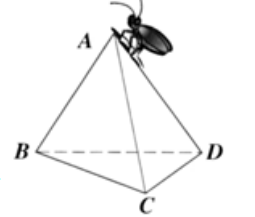
\includegraphics[scale=0.6]{insecte.png}}

A l'aide d'un arbre, calculer les probabilités des événements suivants:

\begin{enumerate}
    \item Le scarabée est en A au bout de trois minutes
    \item Durant les trois premières minutes, le scarabée ne passe jamais au sommet C.
\end{enumerate}

\subsection*{Exercice n°16}

Un commerçant doit livre quatre clients A, B,C et D. On appelle trajet la succession des quatre livraisons.\\
Quel est le nombre de trajets :

\begin{enumerate}
    \item Au total ?
    \item Commençant par le client A ?
    \item Si le commerçant doit livrer A avant B et C ?
\end{enumerate}

\subsection*{Exercice n°17}

Une urne contient 3 jetons: un bleu, un blanc et un rouge.\\
On choisit un jeton, on note sa couleur et on le remet dans l'urne; on choisit un deuxième jeton et on note à nouveau sa couleur.\\
On représente un tirage par un couple dont le premier élément est le premier jeton choisi et le second élément, le deuxième jeton choisi.\\

\begin{enumerate}
    \item Déterminer, à l'aide d'un arbre, l'ensemble de tous les tirages possibles.
    \item Quelle est la probabilité de ne piocher aucune jeton blanc ?
    \item Quelle est la probabilité de piocher au moins un jeton blanc ?
    \item Quelle est la probabilité de piocher deux jetons de même couleur ?
\end{enumerate}

\newpage
\subsection*{Exercice n°18}
En se baladant dans les hautes herbes de la région d'Alola, Sacha réalise qu'il rencontre toujours les quatres même Pokémons:

\begin{center}
    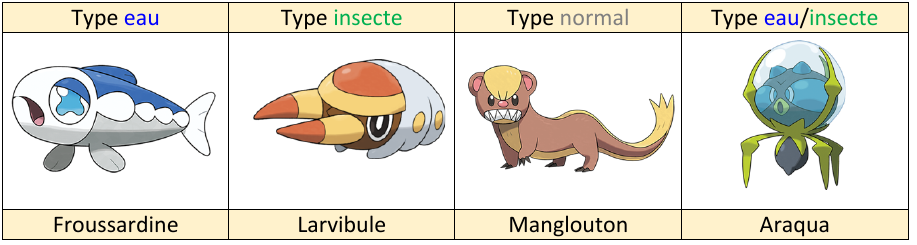
\includegraphics[scale=0.5]{pokemon.png}
\end{center}

Certains Pokémons sont cependant rencontrés plus souvent que les autres.\\
Le professeur Euphorbe affirme que:
\begin{itemize}
    \item 20\% des Pokémons rencontrés sur Alola sont de type normal
    \item 50\% des  Pokémons rencontrés sur Alola sont de type eau
    \item 60\% des Pokémons rencontrés sur Alola sont de type insecte
\end{itemize}

Posons I:\og Rencontrer un Pokémon de type insecte \fg et E:\og Rencontrer un Pokémon de type eau \fg{}

\begin{enumerate}
    \item Associer les événements $I\cap E$, $I \inter \bar{E}$, $\bar{I}\inter E$ et $\bar{I}\inter \bar{E}$ à leurs Pokémons respectifs.
    \item Compléter le tableau suivant et en déduire la probabilité d'apparition de chaque Pokémon.
\begin{center}


\begin{tabular}{|p{2.5cm}|p{4cm}|p{4cm}|p{2.5cm}|} \hline
 & $I$ &$\bar{I}$& Total \\ \hline
$E$&  & & \\ \hline
 $\bar{E}$ & & & \\ \hline
Total & & & 100\\ \hline
\end{tabular} 
   
\end{center}
\end{enumerate}

\subsection*{Exercice n°19}

Un cabinet de recrutement fait passer à des candidats deux examens, l'un est en mathématiques et l'autre en français. L'examen permet de déterminer si le candidat a un niveau satisfaisant ou non dans la matière sur lequel il porte.\\
On dispose des informations suivantes:
\begin{itemize}
    \item 80\% des candidats n'ont pas un niveau satisfaisant en mathématiques;
    \item Les candidats qui ont un niveau satisfaisant en français sont trois fois plus nombreux que ceux qui n'ont pas un niveau satisfaisant en français;
    \item Parmi les candidats dont le niveau en mathématiques est satisfaisant, 50\% ont un niveau satisfaisant en français.
\end{itemize}
On interroge un candidat au hasard et s'intéresse à son niveau en mathématiques et en français.\\
On considère les événements:

\begin{itemize}
    \item M: \og Le candidat a un niveau satisfaisant en mathématiques \fg
    \item F: \og Le candidat a un niveau satisfaisant en français \fg
\end{itemize}

\begin{enumerate}
    \item Compléter le tableau ci-dessous
    
    \begin{center}


\begin{tabular}{|p{2.5cm}|p{4cm}|p{4cm}|p{2.5cm}|} \hline
 & $M$ &$\bar{M}$& Total \\ \hline
$F$&  & & \\ \hline
 $\bar{F}$ & & & \\ \hline
Total & & & 100\\ \hline
\end{tabular} 
   
\end{center}

\item Déterminer la probabilité des événements:
\begin{enumerate}
    \item $\bar{F}$
    \item $\bar{M}$
    \item $\bar{F} \inter \bar{M}$
    \item $\bar{F} \union \bar{M}$
    \item $F \union M$
\end{enumerate}

\end{enumerate}


\subsection*{Exercice n°20}

Soit l'ensemble $\Omega$ constitué des nombres entiers de 1 à 20 inclus. On choisit au hasard un de ces nombres.\\
On considère les quatre événements suivants:

\begin{itemize}
    \item A:\og Le nombre est multiple de 2 \fg{}
    \item B:\og Le nombre est multiple de 4 \fg{}
    \item C:\og Le nombre est multiple de 5 \fg{}
    \item D:\og Le nombre est multiple de 4 mais pas de 2\fg{}
\end{itemize}

\begin{enumerate}
    \item Donner la liste des éléments de $\Omega$.
    \item Lors d'un tirage, l'événement $A$ peut être réalisé pour 10 nombres différents, lesquels ?
    \item L'événement $D$ peut-il être réalisé ?
    \item Décrire en une phrase les éléments de $A\inter C$. Quels tirages sont favorables à $A\inter C$ ?
    \item Mêmes questions pour les événements $B\inter C$ et $\bar{A}\inter \bar{C}$
\end{enumerate}

\subsection*{Exercice n°21}

Chaque lettre du mot \og LIONS \fg est écrite sur un carton et ces cartons sont placés dans un sac. On choisit un carton au hasard, puis, sans le remettre dans le sac, on choisit un second carton placé à droite du premier.\\
On forme ainsi des \og mots \fg de deux lettres

\begin{enumerate}
    \item A l'aide d'un arbre, donner les éléments de l'ensemble $\Omega$ de tous les mots que l'on peut ainsi former. Quel est le nombre des éléments de $\Omega$
    \item On considère les événements suivants :
    \begin{itemize}
        \item A:\og Le mot de deux lettres comporte deux voyelles \fg
        \item B:\og Le mot de deux lettres commence par I \fg
        \item  C:\og Le mot de deux lettres se termine par S \fg
    \end{itemize}
    Décrire en une phrase l'événement $B\inter C$, puis l'événement $A\inter B$ puis $A\union B$
    \item Calculer la probabilité de chacun des événements $A$,$B$,$C$ ,$\bar{A}$, $A\inter B$ et $A\union B$
    \item Retrouver la valeur $p(A\union B)$ par le calcul 
\end{enumerate}

\section{Pour aller plus loin}

\subsection*{Exercice n°22}

Dans une classe de 2nd les langues suivantes sont étudiées: anglais, allemand et espagnol.
Chaque élève étudie au moins une langue et:

\compo{
\begin{itemize}

    \item 5 élèves étudient les trois langues
    \item 8 élèves étudient l'anglais et l'espagnol
    \item 20 élèves étudient l'anglais
    \item 15 élèves étudient l'allemand
\end{itemize}}{\begin{itemize}
    \item 18 élèves étudient l'espagnol
    \item 7 élèves étudient l'anglais et l'allemand
    \item 9 élèves étudient l'allemand et l'espagnol
\end{itemize}}


\begin{center}
\begin{tikzpicture}

\draw(2,0) ellipse (3 and 2);
\draw(-2,0) ellipse (3 and 2);
\draw(0,-2) ellipse (3 and 2);
\draw(-3,0) node{Groupe anglais};
\draw(3,0) node{Groupe espagnol};
\draw(0,-3) node{Groupe allemand};
\end{tikzpicture}
\end{center}

\subsection*{Exercice n°23}

Lors d'une enquête à la sortie du lycée, on a interrogé $60$ élèves. Durant la semaine précédent l'enquête, $35$ avaient lu un livre, $30$ étaient allés au cinéma et, parmi ces derniers, $10$ avaient lu un livre. On interroge un de ces élèves. Déterminer, à l'aide d'un tableau à double entrée, la probabilité des événements suivants ( donner les résultats en fractions):

\begin{itemize}
    \item A: \og Interroger un élève ayant lu un livre\fg
    \item B: \og Interroger un élève qui est allé au cinéma \fg{}
    \item C:\og Interroger un élève ayant lu un livre, mais qui n'est pas allé au cinéma
    \item D: \og Interroger un élève n'ayant ni lu un livre ni vu un film \fg
\end{itemize}

\subsection*{Exercice n°24}

Une entreprise piscicole gère deux bassins.\\











\end{document}